\FloatBarrier
\newtcolorbox{boxA}{
    boxrule = 1.5pt,
    colframe = black %
}

\section{Automatic and Human Evaluation}
\begin{figure}[!ht]
    \centering
    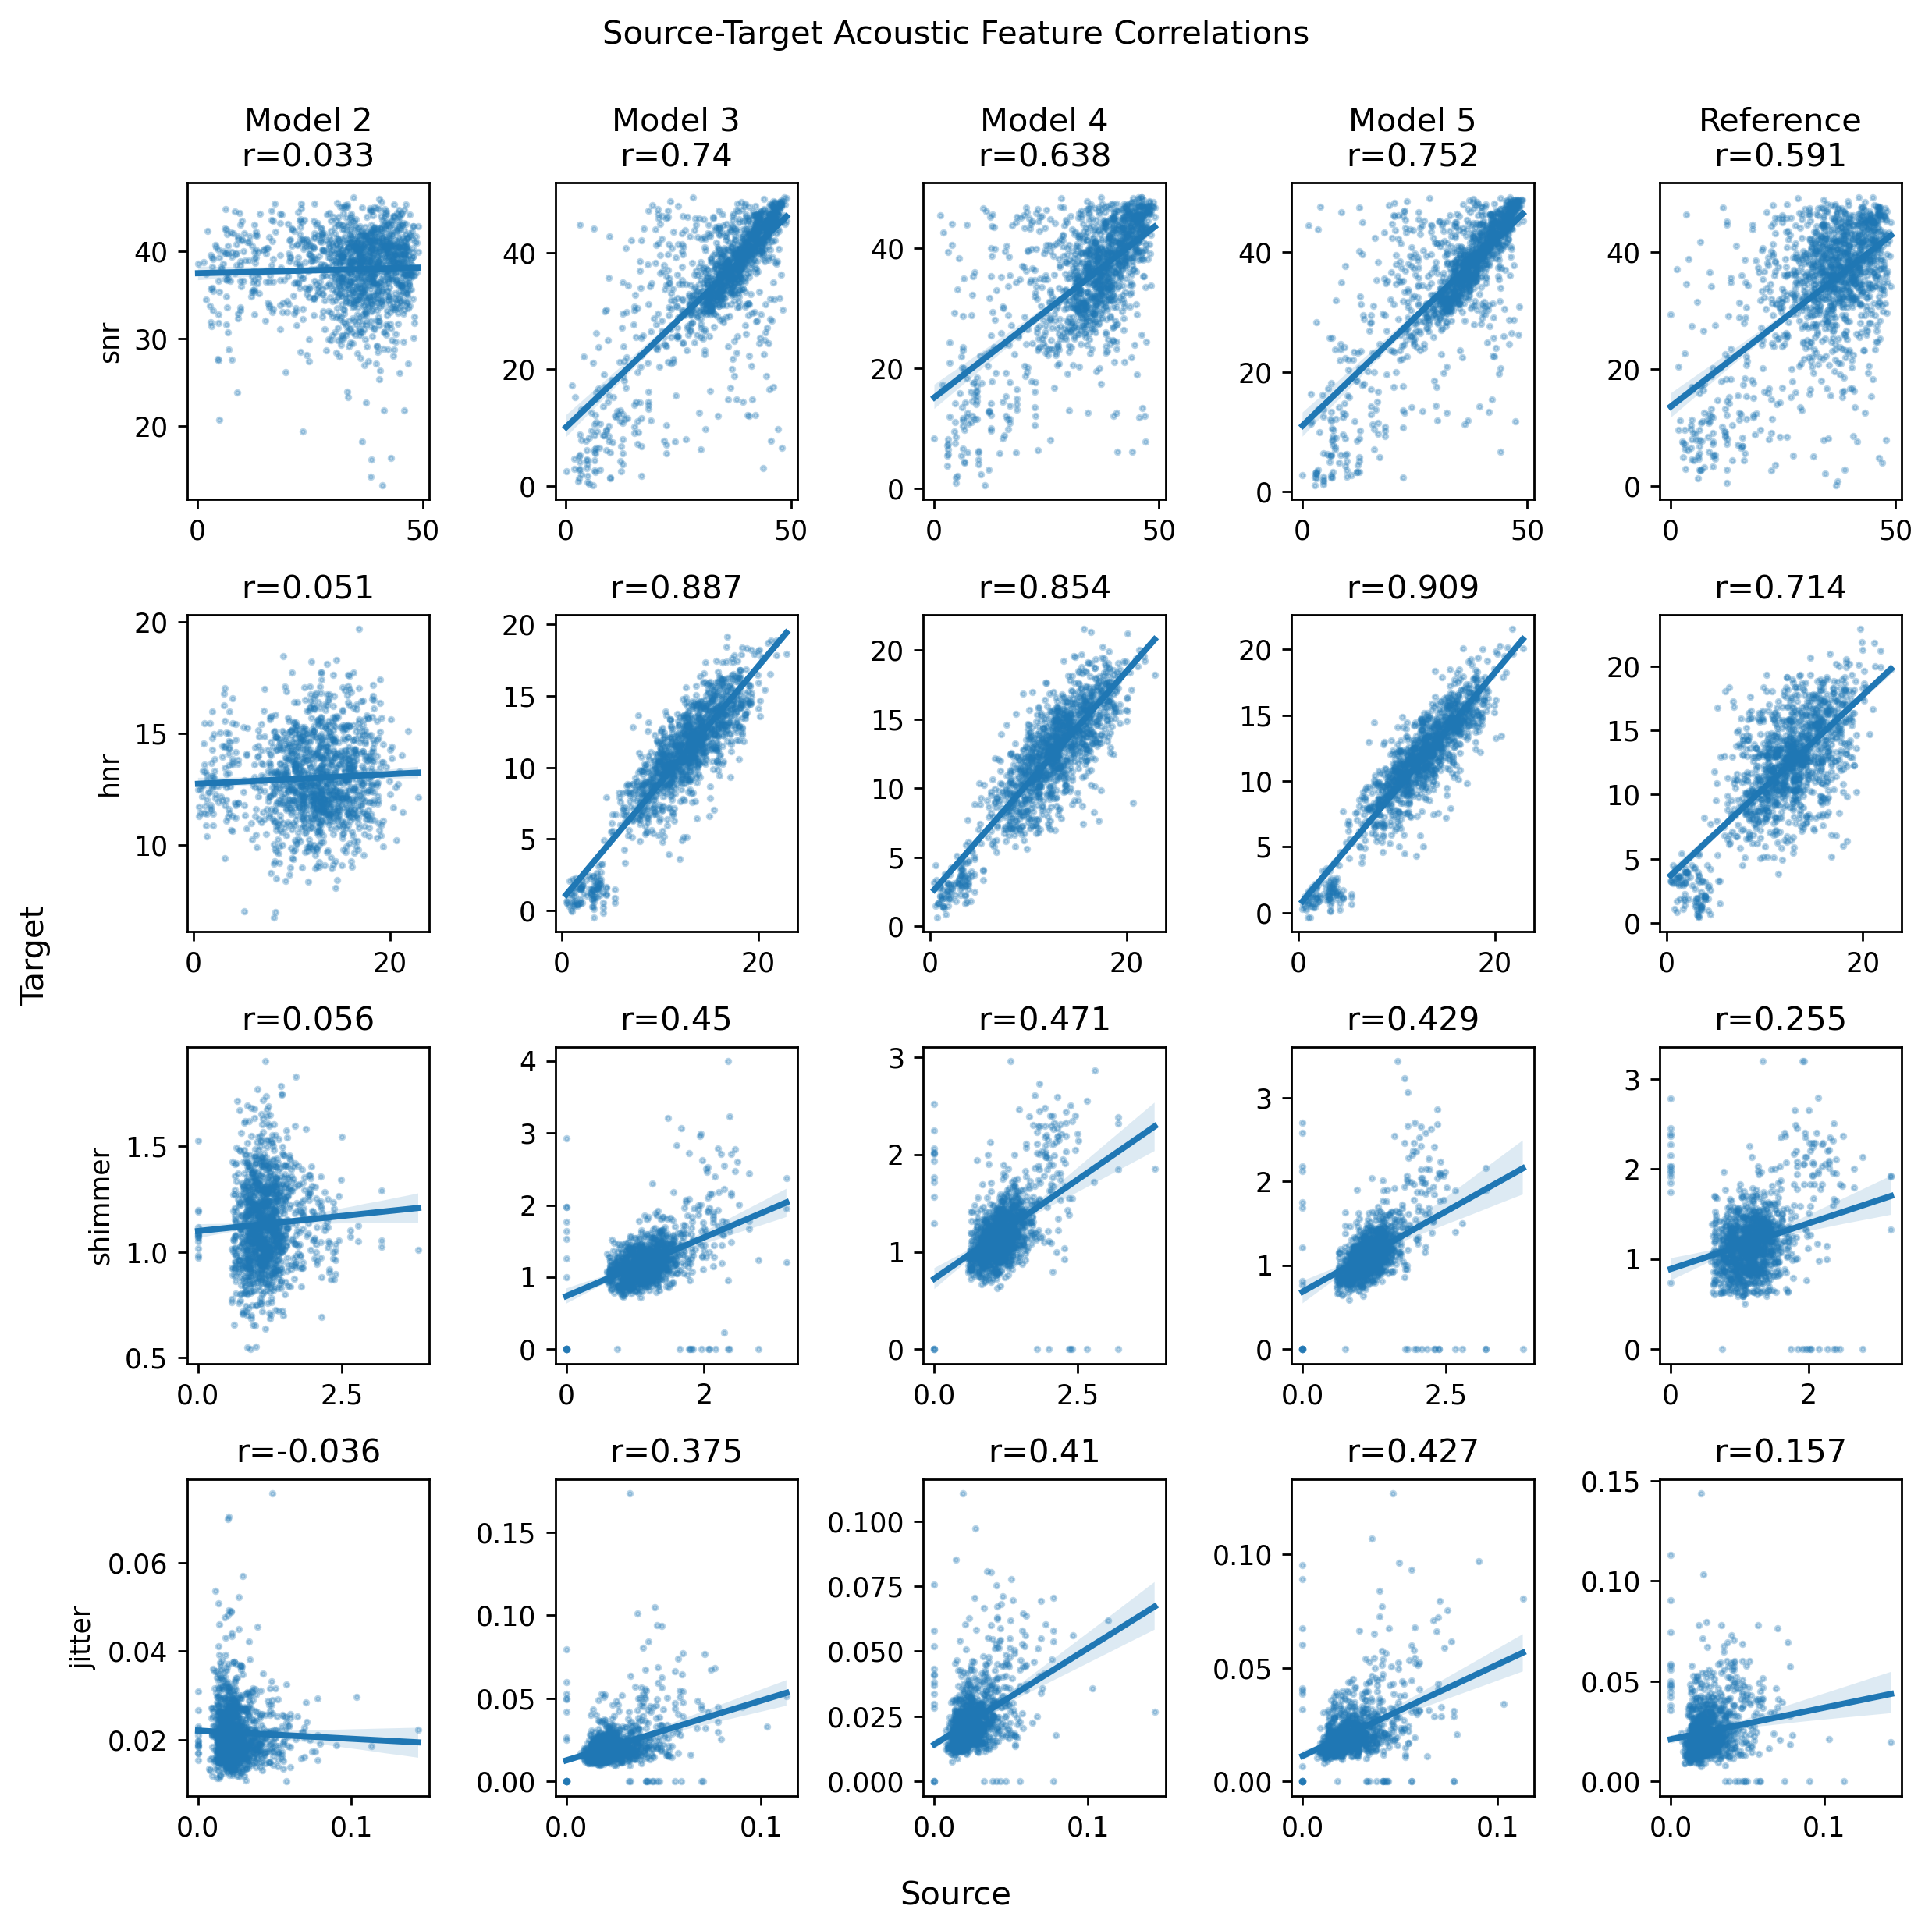
\includegraphics[width=0.8\linewidth]{figures/evaluation/snr.hnr.shimmer.jitter-pointwise-correlations.png}
    \caption{Acoustic correlates of noise (SNR, HNR, shimmer, and jitter) pointwise correlation between source and target outputs by model.}
    \label{fig:snr.hnr.shimmer.jitter-pointwise-correlations}
\end{figure}

\begin{figure}[!ht]
    \centering
    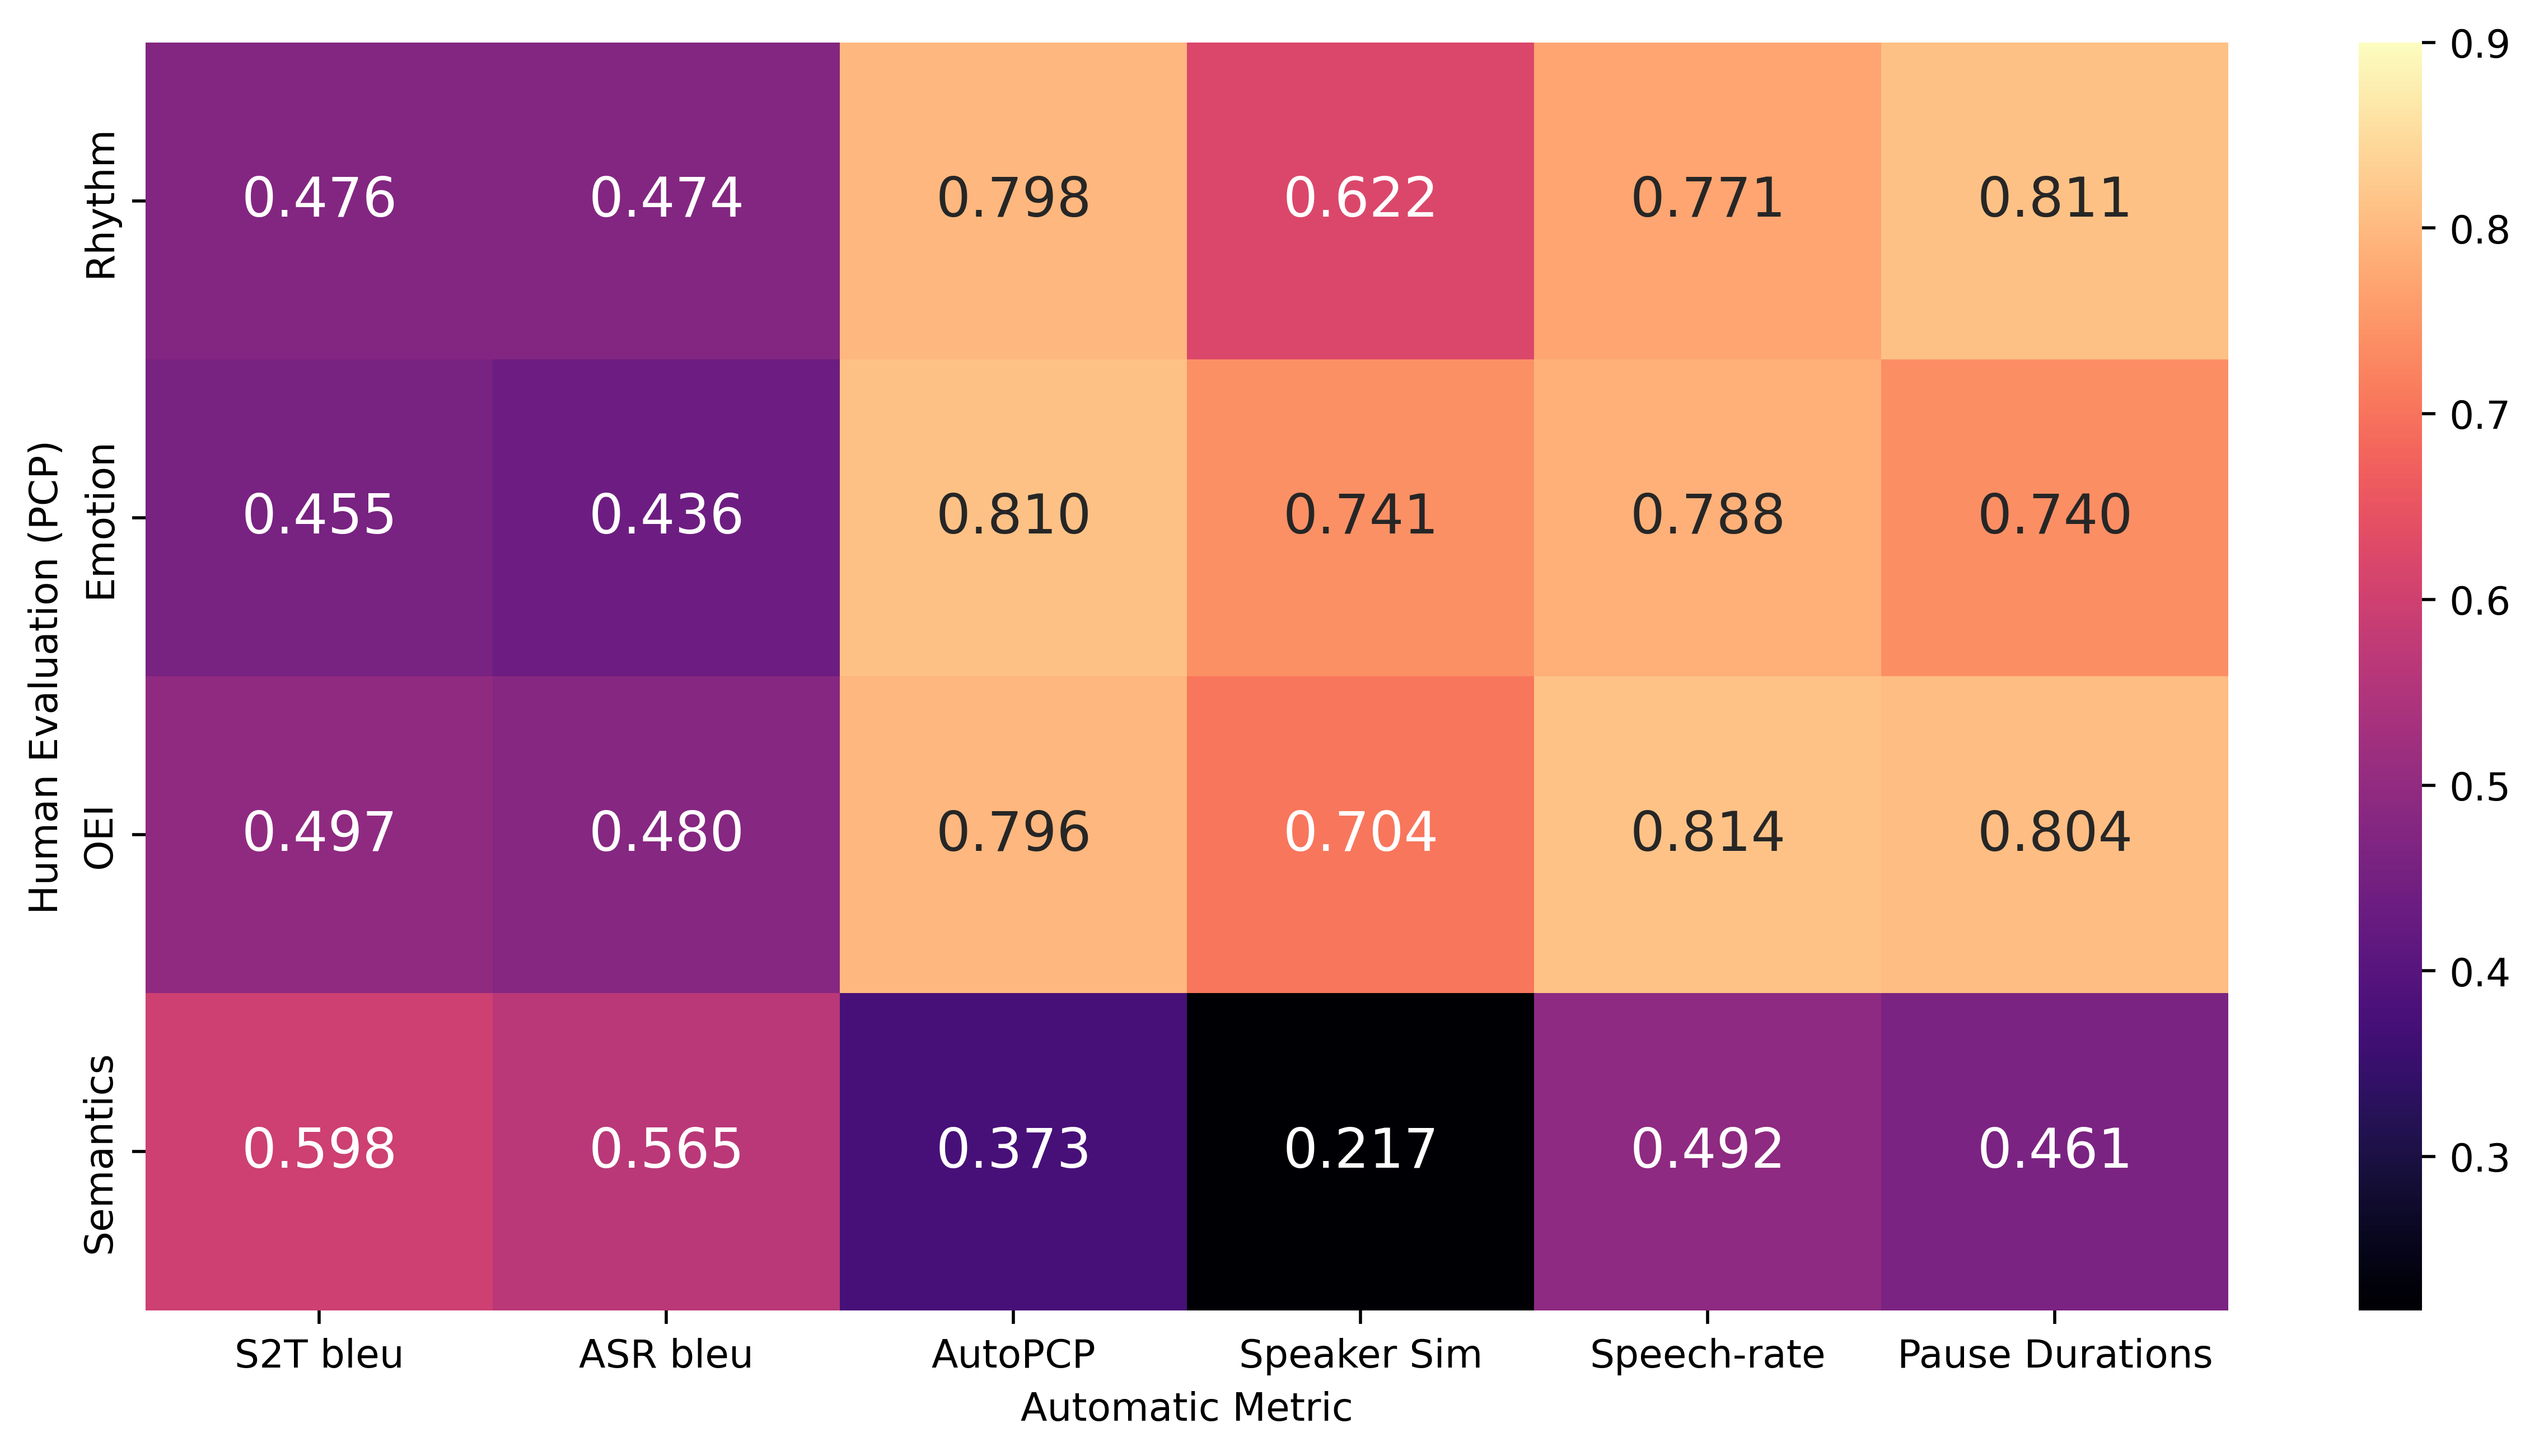
\includegraphics[width=0.8\linewidth]{figures/evaluation/spearman_r_matrix.png}
    \caption{\textbf{Human Evaluation (PCP) metrics correlation to Expressivity automatic metrics.} We the Spearman correlation between all pairwise combinations of human- and automatic-metrics.}
    \label{fig:metrics_spearman_matrix}
\end{figure}

\subsection{Human Evaluation}

\begin{table}[!ht]
\tiny
\centering
\begin{tabular}{c|ccc|ccc}
\hline
cmn->eng & \multicolumn{3}{c|}{mDral} & \multicolumn{3}{c|}{mExpresso}\\
\hline
ID & Emotion & OEI & Rhythm & Emotion & OEI & Rhythm \\
\hline
Reference & 3.61 (0.22) & 3.30 (0.16) & 3.65 (0.21) & 3.20 (0.10) & 3.15 (0.10) & 3.42 (0.09)\\
5 & 3.64 (0.17) & 3.49 (0.23) & 3.49 (0.24) & 3.60 (0.09) & 3.46 (0.10) & 3.64 (0.08)\\
4 & 3.90 (0.10) & 3.39 (0.22) & 3.50 (0.22) & 3.65 (0.09) & 3.47 (0.10) & 3.65 (0.09)\\
3 & 3.49 (0.28) & 3.39 (0.28) & 3.29 (0.34) & 2.73 (0.16) & 2.63 (0.14) & 2.45 (0.18)\\
2 & 2.59 (0.36) & 2.90 (0.31) & 2.90 (0.39) & 2.11 (0.14) & 2.24 (0.12) & 2.24 (0.14)\\
\hline
deu->eng & \multicolumn{3}{c|}{mDral} & \multicolumn{3}{c|}{mExpresso}\\
\hline
ID & Emotion & OEI & Rhythm & Emotion & OEI & Rhythm \\
\hline
Reference & 3.89 (0.02) & 3.88 (0.02) & 3.79 (0.03) & 3.12 (0.03) & 3.25 (0.03) & 3.33 (0.02)\\
5 & 3.61 (0.05) & 3.65 (0.04) & 3.59 (0.04) & 3.64 (0.02) & 3.60 (0.02) & 3.61 (0.02)\\
4 & 3.68 (0.04) & 3.65 (0.04) & 3.69 (0.04) & 3.68 (0.02) & 3.60 (0.02) & 3.61 (0.02)\\
3 & 3.36 (0.05) & 3.32 (0.05) & 3.06 (0.06) & 3.13 (0.03) & 3.03 (0.03) & 2.92 (0.03)\\
2 & 2.86 (0.06) & 2.89 (0.06) & 2.83 (0.06) & 2.47 (0.03) & 2.60 (0.03) & 2.58 (0.03)\\
\hline
fra->eng & \multicolumn{3}{c|}{mDral} & \multicolumn{3}{c|}{mExpresso}\\
\hline
ID & Emotion & OEI & Rhythm & Emotion & OEI & Rhythm \\
\hline
Reference & 3.77 (0.15) & 3.77 (0.15) & 3.89 (0.11) & 3.24 (0.17) & 3.13 (0.17) & 3.54 (0.18)\\
5 & 3.89 (0.11) & 3.45 (0.18) & 4.00 (0.00) & 3.13 (0.15) & 3.30 (0.14) & 3.54 (0.16)\\
4 & 3.34 (0.24) & 3.23 (0.22) & 3.67 (0.17) & 3.09 (0.18) & 2.82 (0.14) & 3.56 (0.17)\\
3 & 2.89 (0.32) & 3.01 (0.24) & 3.33 (0.30) & 2.82 (0.22) & 2.62 (0.14) & 2.88 (0.25)\\
2 & 2.42 (0.38) & 2.65 (0.29) & 3.10 (0.35) & 2.48 (0.20) & 2.51 (0.16) & 2.55 (0.24)\\
\hline
ita->eng & \multicolumn{3}{c|}{mDral} & \multicolumn{3}{c|}{mExpresso}\\
\hline
ID & Emotion & OEI & Rhythm & Emotion & OEI & Rhythm \\
\hline
Reference & 3.87 (0.03) & 3.68 (0.04) & 3.80 (0.03) & 3.49 (0.03) & 3.38 (0.03) & 3.56 (0.03)\\
5 & 3.56 (0.06) & 3.49 (0.05) & 3.61 (0.05) & 3.67 (0.03) & 3.46 (0.03) & 3.50 (0.03)\\
4 & 3.55 (0.05) & 3.39 (0.05) & 3.53 (0.05) & 3.63 (0.03) & 3.42 (0.03) & 3.47 (0.03)\\
3 & 3.33 (0.06) & 3.06 (0.06) & 3.06 (0.07) & 3.39 (0.03) & 3.20 (0.03) & 3.15 (0.04)\\
2 & 3.01 (0.07) & 2.87 (0.06) & 2.81 (0.07) & 2.74 (0.04) & 2.76 (0.03) & 2.91 (0.04)\\
\hline
spa->eng & \multicolumn{3}{c|}{mDral} & \multicolumn{3}{c|}{mExpresso}\\
\hline
ID & Emotion & OEI & Rhythm & Emotion & OEI & Rhythm \\
\hline
Reference & 3.96 (0.02) & 3.92 (0.02) & 3.96 (0.02) & 3.85 (0.02) & 3.77 (0.02) & 3.86 (0.01)\\
5 & 3.44 (0.06) & 3.34 (0.06) & 3.54 (0.05) & 3.76 (0.02) & 3.48 (0.02) & 3.50 (0.03)\\
4 & 3.55 (0.06) & 3.44 (0.06) & 3.57 (0.05) & 3.72 (0.02) & 3.44 (0.03) & 3.48 (0.03)\\
3 & 3.29 (0.07) & 3.12 (0.06) & 3.30 (0.07) & 3.41 (0.03) & 2.97 (0.03) & 2.85 (0.04)\\
2 & 2.74 (0.09) & 2.64 (0.07) & 2.86 (0.08) & 2.39 (0.04) & 2.38 (0.03) & 2.51 (0.04)\\
\hline
\end{tabular}
\caption{\label{tab:pcp_human_evaluation_full_table} Average median PCP scores with standard errors aggregated to the language direction by dataset level.}
\end{table}

\begin{table}[!ht]
\tiny
\centering
\begin{tabular}{c|ccc|ccc|ccc}
\hline
deu->eng & \multicolumn{3}{c|}{FLEURS} & \multicolumn{3}{c|}{mDral} & \multicolumn{3}{c|}{mExpresso}\\
\hline
ID & Clar. & Nat. & Qual. & Clar. & Nat. & Qual. & Clar. & Nat. & Qual. \\
\hline
Reference & 4.84 & 4.95 & 3.51 & 4.94 & 4.87 & 4.94 & 5.00 & 5.00 & 5.00\\
5 & 4.79 & 4.51 & 4.15 & 4.87 & 3.74 & 4.54 & 4.94 & 4.31 & 4.56\\
4 & 4.89 & 4.31 & 4.95 & 4.87 & 3.67 & 4.61 & 5.00 & 4.49 & 4.88\\
3 & 4.85 & 4.53 & 4.11 & 4.67 & 4.41 & 4.14 & 4.69 & 4.37 & 4.43\\
2 & 4.90 & 4.69 & 4.37 & 4.80 & 4.54 & 4.66 & 4.94 & 4.43 & 4.51\\
\hline
fra->eng & \multicolumn{3}{c|}{FLEURS} & \multicolumn{3}{c|}{mDral} & \multicolumn{3}{c|}{mExpresso}\\
\hline
ID & Clar. & Nat. & Qual. & Clar. & Nat. & Qual. & Clar. & Nat. & Qual. \\
\hline
Reference & 4.34 & 4.51 & 3.46 & 4.36 & 4.49 & 4.63 & 4.93 & 4.14 & 5.00\\
5 & 4.72 & 3.77 & 4.05 & 4.51 & 3.65 & 4.01 & 4.63 & 3.25 & 3.89\\
4 & 4.76 & 3.90 & 4.47 & 4.93 & 3.50 & 4.57 & 4.75 & 3.46 & 4.39\\
3 & 4.33 & 4.00 & 3.91 & 4.57 & 4.07 & 3.92 & 4.43 & 3.79 & 4.15\\
2 & 4.61 & 4.09 & 4.13 & 4.93 & 4.15 & 4.42 & 4.60 & 4.01 & 4.40\\
\hline
ita->eng & \multicolumn{3}{c|}{FLEURS} & \multicolumn{3}{c|}{mDral} & \multicolumn{3}{c|}{mExpresso}\\
\hline
ID & Clar. & Nat. & Qual. & Clar. & Nat. & Qual. & Clar. & Nat. & Qual. \\
\hline
Reference & 4.78 & 4.89 & 3.77 & 4.32 & 4.81 & 4.42 & 4.97 & 4.52 & 4.95\\
5 & 4.88 & 3.51 & 4.30 & 4.74 & 3.69 & 4.28 & 4.77 & 4.17 & 4.29\\
4 & 4.89 & 3.39 & 4.77 & 4.83 & 3.85 & 4.58 & 4.89 & 4.21 & 4.56\\
3 & 4.89 & 4.41 & 4.32 & 4.73 & 4.24 & 4.23 & 4.71 & 4.37 & 4.22\\
2 & 4.89 & 4.38 & 4.23 & 4.93 & 4.31 & 4.44 & 4.87 & 4.36 & 4.51\\
\hline
spa->eng & \multicolumn{3}{c|}{FLEURS} & \multicolumn{3}{c|}{mDral} & \multicolumn{3}{c|}{mExpresso}\\
\hline
ID & Clar. & Nat. & Qual. & Clar. & Nat. & Qual. & Clar. & Nat. & Qual. \\
\hline
Reference & 4.77 & 4.83 & 3.84 & 4.32 & 4.50 & 4.33 & 4.90 & 4.43 & 4.93\\
5 & 4.39 & 3.60 & 3.63 & 4.39 & 3.74 & 4.03 & 4.49 & 3.73 & 4.15\\
4 & 4.64 & 3.68 & 4.33 & 4.67 & 3.97 & 4.56 & 4.73 & 3.95 & 4.61\\
3 & 4.45 & 4.12 & 3.63 & 4.37 & 4.03 & 4.05 & 4.54 & 4.12 & 4.21\\
2 & 4.63 & 4.11 & 4.22 & 4.73 & 4.28 & 4.54 & 4.69 & 4.26 & 4.46\\
\hline
eng->cmn & \multicolumn{3}{c|}{FLEURS} & \multicolumn{3}{c|}{mDral} & \multicolumn{3}{c|}{mExpresso}\\
\hline
ID & Clar. & Nat. & Qual. & Clar. & Nat. & Qual. & Clar. & Nat. & Qual. \\
\hline
Reference & 4.65 & 4.88 & 4.48 & 4.53 & 4.77 & 4.60 & 4.41 & 4.55 & 4.50\\
5 & 2.09 & 2.68 & 2.15 & 3.78 & 3.75 & 3.72 & 3.50 & 3.21 & 3.57\\
4 & 3.12 & 3.38 & 3.28 & 4.18 & 4.08 & 4.33 & 3.86 & 3.37 & 4.30\\
3 & 2.23 & 2.90 & 2.35 & 3.98 & 4.12 & 3.88 & 3.91 & 3.94 & 3.97\\
2 & 4.55 & 3.67 & 4.67 & 4.56 & 3.58 & 4.64 & 4.59 & 3.63 & 4.69\\
\hline
eng->deu & \multicolumn{3}{c|}{FLEURS} & \multicolumn{3}{c|}{mDral} & \multicolumn{3}{c|}{mExpresso}\\
\hline
ID & Clar. & Nat. & Qual. & Clar. & Nat. & Qual. & Clar. & Nat. & Qual. \\
\hline
Reference & 3.69 & 3.87 & 3.69 & 4.11 & 4.42 & 4.02 & 3.95 & 3.67 & 3.68\\
5 & 3.07 & 3.59 & 2.41 & 3.84 & 3.35 & 3.30 & 3.67 & 3.23 & 3.19\\
4 & 3.29 & 3.68 & 2.67 & 4.24 & 3.53 & 3.84 & 4.21 & 3.39 & 4.21\\
3 & 2.92 & 4.01 & 2.46 & 3.86 & 3.79 & 3.42 & 3.71 & 3.73 & 3.43\\
2 & 4.16 & 3.32 & 4.19 & 4.38 & 3.42 & 4.10 & 4.25 & 3.42 & 4.25\\
\hline
eng->fra & \multicolumn{3}{c|}{FLEURS} & \multicolumn{3}{c|}{mDral} & \multicolumn{3}{c|}{mExpresso}\\
\hline
ID & Clar. & Nat. & Qual. & Clar. & Nat. & Qual. & Clar. & Nat. & Qual. \\
\hline
Reference & 4.07 & 4.59 & 3.77 & 4.33 & 4.51 & 4.07 & 4.23 & 4.24 & 3.98\\
5 & 3.41 & 3.69 & 2.36 & 4.16 & 3.76 & 3.37 & 4.12 & 3.22 & 3.53\\
4 & 3.72 & 3.73 & 2.90 & 4.39 & 3.89 & 3.92 & 4.28 & 3.29 & 4.19\\
3 & 3.22 & 3.84 & 2.30 & 3.88 & 3.97 & 3.43 & 3.87 & 3.85 & 3.58\\
2 & 4.02 & 3.30 & 4.11 & 4.27 & 3.61 & 4.25 & 4.13 & 3.50 & 4.26\\
\hline
eng->ita & \multicolumn{3}{c|}{FLEURS} & \multicolumn{3}{c|}{mDral} & \multicolumn{3}{c|}{mExpresso}\\
\hline
ID & Clar. & Nat. & Qual. & Clar. & Nat. & Qual. & Clar. & Nat. & Qual. \\
\hline
Reference & 4.73 & 4.50 & 4.14 & 4.24 & 4.78 & 4.27 & 4.64 & 4.65 & 4.45\\
5 & 2.94 & 3.67 & 2.50 & 4.34 & 3.68 & 3.73 & 4.27 & 3.20 & 3.83\\
4 & 3.55 & 3.71 & 3.00 & 4.44 & 3.71 & 4.19 & 4.42 & 3.21 & 4.42\\
3 & 2.97 & 3.72 & 2.38 & 4.19 & 4.00 & 3.81 & 4.13 & 3.73 & 3.94\\
2 & 4.39 & 4.00 & 4.59 & 4.41 & 3.70 & 4.57 & 4.44 & 3.88 & 4.62\\
\hline
eng->spa & \multicolumn{3}{c|}{FLEURS} & \multicolumn{3}{c|}{mDral} & \multicolumn{3}{c|}{mExpresso}\\
\hline
ID & Clar. & Nat. & Qual. & Clar. & Nat. & Qual. & Clar. & Nat. & Qual. \\
\hline
Reference & 4.65 & 4.77 & 3.94 & 4.51 & 4.55 & 4.21 & 4.76 & 4.26 & 4.62\\
5 & 3.41 & 3.75 & 2.27 & 4.57 & 3.88 & 3.65 & 4.58 & 3.52 & 3.79\\
4 & 4.10 & 3.86 & 3.02 & 4.61 & 3.88 & 4.03 & 4.68 & 3.57 & 4.50\\
3 & 3.34 & 3.81 & 2.30 & 4.41 & 4.11 & 3.69 & 4.46 & 4.16 & 3.91\\
2 & 4.60 & 4.25 & 4.40 & 4.68 & 4.19 & 4.62 & 4.67 & 4.20 & 4.61\\
\hline
\end{tabular}
\caption{\label{tab:mos_human_evaluation_full_table_mu}Average median MOS scores aggregated to the language direction by dataset level.}
\end{table}

\begin{table}[!ht]
\tiny
\centering
\begin{tabular}{c|ccc|ccc|ccc}
\hline
deu->eng & \multicolumn{3}{c|}{FLEURS} & \multicolumn{3}{c|}{mDral} & \multicolumn{3}{c|}{mExpresso}\\
\hline
ID & Clar. & Nat. & Qual. & Clar. & Nat. & Qual. & Clar. & Nat. & Qual. \\
\hline
Reference & 0.11 & 0.05 & 0.21 & 0.07 & 0.09 & 0.07 & 0.00 & 0.00 & 0.00\\
5 & 0.13 & 0.16 & 0.14 & 0.09 & 0.31 & 0.13 & 0.06 & 0.17 & 0.12\\
4 & 0.07 & 0.18 & 0.05 & 0.08 & 0.19 & 0.16 & 0.00 & 0.13 & 0.08\\
3 & 0.08 & 0.16 & 0.10 & 0.18 & 0.21 & 0.21 & 0.18 & 0.15 & 0.13\\
2 & 0.07 & 0.15 & 0.11 & 0.11 & 0.19 & 0.13 & 0.06 & 0.19 & 0.16\\
\hline
fra->eng & \multicolumn{3}{c|}{FLEURS} & \multicolumn{3}{c|}{mDral} & \multicolumn{3}{c|}{mExpresso}\\
\hline
ID & Clar. & Nat. & Qual. & Clar. & Nat. & Qual. & Clar. & Nat. & Qual. \\
\hline
Reference & 0.18 & 0.17 & 0.16 & 0.19 & 0.20 & 0.13 & 0.05 & 0.15 & 0.00\\
5 & 0.10 & 0.21 & 0.16 & 0.17 & 0.32 & 0.26 & 0.14 & 0.19 & 0.11\\
4 & 0.09 & 0.17 & 0.11 & 0.07 & 0.29 & 0.14 & 0.10 & 0.19 & 0.09\\
3 & 0.13 & 0.13 & 0.17 & 0.17 & 0.30 & 0.23 & 0.11 & 0.17 & 0.12\\
2 & 0.11 & 0.18 & 0.10 & 0.07 & 0.25 & 0.14 & 0.13 & 0.17 & 0.13\\
\hline
ita->eng & \multicolumn{3}{c|}{FLEURS} & \multicolumn{3}{c|}{mDral} & \multicolumn{3}{c|}{mExpresso}\\
\hline
ID & Clar. & Nat. & Qual. & Clar. & Nat. & Qual. & Clar. & Nat. & Qual. \\
\hline
Reference & 0.05 & 0.03 & 0.10 & 0.09 & 0.04 & 0.06 & 0.02 & 0.06 & 0.03\\
5 & 0.03 & 0.08 & 0.05 & 0.06 & 0.09 & 0.06 & 0.05 & 0.09 & 0.06\\
4 & 0.03 & 0.08 & 0.04 & 0.05 & 0.09 & 0.05 & 0.03 & 0.07 & 0.05\\
3 & 0.03 & 0.06 & 0.05 & 0.05 & 0.08 & 0.06 & 0.06 & 0.07 & 0.06\\
2 & 0.03 & 0.06 & 0.05 & 0.03 & 0.06 & 0.06 & 0.04 & 0.06 & 0.05\\
\hline
spa->eng & \multicolumn{3}{c|}{FLEURS} & \multicolumn{3}{c|}{mDral} & \multicolumn{3}{c|}{mExpresso}\\
\hline
ID & Clar. & Nat. & Qual. & Clar. & Nat. & Qual. & Clar. & Nat. & Qual. \\
\hline
Reference & 0.05 & 0.04 & 0.08 & 0.07 & 0.07 & 0.07 & 0.03 & 0.07 & 0.03\\
5 & 0.06 & 0.08 & 0.08 & 0.06 & 0.08 & 0.07 & 0.06 & 0.09 & 0.06\\
4 & 0.05 & 0.08 & 0.07 & 0.05 & 0.08 & 0.06 & 0.04 & 0.08 & 0.05\\
3 & 0.06 & 0.07 & 0.07 & 0.08 & 0.08 & 0.07 & 0.06 & 0.07 & 0.07\\
2 & 0.05 & 0.07 & 0.06 & 0.05 & 0.06 & 0.06 & 0.04 & 0.06 & 0.05\\
\hline
eng->cmn & \multicolumn{3}{c|}{FLEURS} & \multicolumn{3}{c|}{mDral} & \multicolumn{3}{c|}{mExpresso}\\
\hline
ID & Clar. & Nat. & Qual. & Clar. & Nat. & Qual. & Clar. & Nat. & Qual. \\
\hline
Reference & 0.04 & 0.03 & 0.04 & 0.05 & 0.03 & 0.04 & 0.03 & 0.02 & 0.03\\
5 & 0.08 & 0.10 & 0.08 & 0.07 & 0.07 & 0.06 & 0.03 & 0.03 & 0.03\\
4 & 0.08 & 0.08 & 0.08 & 0.06 & 0.07 & 0.05 & 0.03 & 0.03 & 0.03\\
3 & 0.09 & 0.11 & 0.09 & 0.06 & 0.07 & 0.06 & 0.03 & 0.03 & 0.03\\
2 & 0.05 & 0.06 & 0.04 & 0.05 & 0.07 & 0.04 & 0.02 & 0.03 & 0.02\\
\hline
eng->deu & \multicolumn{3}{c|}{FLEURS} & \multicolumn{3}{c|}{mDral} & \multicolumn{3}{c|}{mExpresso}\\
\hline
ID & Clar. & Nat. & Qual. & Clar. & Nat. & Qual. & Clar. & Nat. & Qual. \\
\hline
Reference & 0.12 & 0.13 & 0.13 & 0.11 & 0.10 & 0.11 & 0.07 & 0.07 & 0.06\\
5 & 0.15 & 0.14 & 0.14 & 0.12 & 0.10 & 0.08 & 0.06 & 0.06 & 0.05\\
4 & 0.17 & 0.14 & 0.20 & 0.11 & 0.13 & 0.09 & 0.06 & 0.07 & 0.05\\
3 & 0.11 & 0.11 & 0.12 & 0.11 & 0.11 & 0.10 & 0.06 & 0.05 & 0.06\\
2 & 0.12 & 0.14 & 0.11 & 0.10 & 0.11 & 0.11 & 0.06 & 0.07 & 0.05\\
\hline
eng->fra & \multicolumn{3}{c|}{FLEURS} & \multicolumn{3}{c|}{mDral} & \multicolumn{3}{c|}{mExpresso}\\
\hline
ID & Clar. & Nat. & Qual. & Clar. & Nat. & Qual. & Clar. & Nat. & Qual. \\
\hline
Reference & 0.06 & 0.04 & 0.06 & 0.06 & 0.05 & 0.05 & 0.03 & 0.03 & 0.03\\
5 & 0.08 & 0.07 & 0.08 & 0.06 & 0.06 & 0.05 & 0.03 & 0.04 & 0.03\\
4 & 0.07 & 0.06 & 0.08 & 0.05 & 0.07 & 0.05 & 0.03 & 0.04 & 0.03\\
3 & 0.09 & 0.07 & 0.08 & 0.07 & 0.07 & 0.06 & 0.03 & 0.03 & 0.03\\
2 & 0.06 & 0.06 & 0.05 & 0.07 & 0.07 & 0.05 & 0.03 & 0.03 & 0.02\\
\hline
eng->ita & \multicolumn{3}{c|}{FLEURS} & \multicolumn{3}{c|}{mDral} & \multicolumn{3}{c|}{mExpresso}\\
\hline
ID & Clar. & Nat. & Qual. & Clar. & Nat. & Qual. & Clar. & Nat. & Qual. \\
\hline
Reference & 0.03 & 0.05 & 0.05 & 0.06 & 0.03 & 0.05 & 0.02 & 0.02 & 0.02\\
5 & 0.09 & 0.07 & 0.07 & 0.04 & 0.06 & 0.05 & 0.02 & 0.04 & 0.02\\
4 & 0.08 & 0.06 & 0.08 & 0.05 & 0.06 & 0.04 & 0.02 & 0.04 & 0.02\\
3 & 0.10 & 0.08 & 0.08 & 0.05 & 0.05 & 0.05 & 0.03 & 0.04 & 0.02\\
2 & 0.06 & 0.06 & 0.04 & 0.05 & 0.06 & 0.04 & 0.03 & 0.03 & 0.02\\
\hline
eng->spa & \multicolumn{3}{c|}{FLEURS} & \multicolumn{3}{c|}{mDral} & \multicolumn{3}{c|}{mExpresso}\\
\hline
ID & Clar. & Nat. & Qual. & Clar. & Nat. & Qual. & Clar. & Nat. & Qual. \\
\hline
Reference & 0.04 & 0.03 & 0.06 & 0.05 & 0.05 & 0.06 & 0.02 & 0.03 & 0.02\\
5 & 0.09 & 0.07 & 0.07 & 0.04 & 0.06 & 0.06 & 0.02 & 0.03 & 0.02\\
4 & 0.07 & 0.06 & 0.07 & 0.04 & 0.06 & 0.05 & 0.02 & 0.03 & 0.02\\
3 & 0.09 & 0.08 & 0.07 & 0.06 & 0.06 & 0.05 & 0.03 & 0.03 & 0.02\\
2 & 0.04 & 0.06 & 0.04 & 0.05 & 0.06 & 0.04 & 0.02 & 0.03 & 0.02\\
\hline
\end{tabular}
\caption{\label{tab:mos_human_evaluation_full_table_se} Standard error of average median MOS scores aggregated to the language direction by dataset level.}
\end{table}

\FloatBarrier
\subsection{Prosodic Consistency Protocol (PCP)}
\label{sec:PCP_protocol_text}

Below, we provide the complete text for the updated Prosodic Consistency Protocol we used for human evaluation in the current study. Note that we have tried to reproduce orthographic markers such as bolding and italicization. For clarity, all Likert response options are single-choice (an annotator may only select one item from i. - iv.).

\subsubsection{Overview}
In this task, you will listen to pairs of audio segments. Each pair will consist of one \{LANG\_1\} segment and one \{LANG\_2\} segment. 

Our goal is to know how similar the two segments (utterances) are perceived in terms of:

\begin{enumerate}
    \item Semantics/Meaning
    \item Emotion
    \item Rhythm
    \item Overall expressive intent
\end{enumerate}

Different languages have distinct speech patterns related to the aspects mentioned above. When comparing expressivity in different languages, we want to determine if the expressive qualities in \{LANG\_1\} convey \textbf{similar information} as in \{LANG\_2\}.

By “overall expressive intent,” we mean the \textbf{overall impact and manner in which the speaker spoke the sentence}. To rate similarity in expressive intent between two audio files, consider aspects like emphasis, tone, rhythm, and the speaker's emotional state combined.

All of the dimensions are explained in more detail below.

\subsubsection{Semantics}
\textbf{The semantics} of an utterance refers to the literal meaning of the words disregarding the manner in which they are spoken. 

\begin{boxA}
\textit{Example:}
The sentence “There is a green apple” in English has a different meaning from “Hay una manzana roja” (“There is a red apple”) in Spanish.
\end{boxA}

Question: Do the two segments have a similar meaning?
\begin{enumerate}
    \item The two segments are \textbf{completely different} in their meaning— \textit{they refer to different objects, actions, or concepts and the relationships between them.}
    \item The two segments are \textbf{mostly different} in their meaning, but share some similarities—\textit{there are some important differences in the meaning of the two segments, although one or more objects, actions or concepts may appear in both sentences.}
    \item The two segments are \textbf{mostly similar} in their meaning, but have some differences - \textit{they could be paraphrases of one another.}
    \item The two segments are \textbf{completely similar} in their meaning—\textit{they are exact translations of one another.}
\end{enumerate}

\subsubsection{Emotion}
\textbf{Emotion} describes the overall feeling of the speaker while they are talking.
\begin{boxA}
\textit{Example:}
A speaker may sound angry, pleased, happy, or confused (to name just a few emotions) while speaking. Consider whether you could imagine the two speakers making similar facial expressions while speaking or whether you could apply the same description of their emotions. 
\end{boxA}
Question: Do the two segments sound similar in the speaker’s emotional state?
\begin{enumerate}
    \item The two segments sound \textbf{completely different} in the emotions conveyed - basically none of the emotion aspects are shared.
    \textit{For example, while one utterance might sound very happy throughout, the other utterance might sound neutral throughout.}
    \item The two segments are \textbf{mostly different}, but share some similarities in terms of emotion.
    \textit{For example, while one utterance might sound happy throughout, the other utterance might sound neutral throughout and happy just at the end.}
    \item The two segments are \textbf{mostly similar} in emotion, but have some differences.
    \textit{For example, both utterances might share the same emotion or mix of emotions, but the emotions are more pronounced in one compared to the other (one segment sounds very happy while the other is subtly pleased).}
    \item The two segments sound \textbf{completely similar} in the emotions conveyed— basically all of the emotion aspects are shared.
    \textit{For example, both utterances sound very happy to the same extent and this is expressed similarly throughout.}
\end{enumerate}

\subsubsection{Rhythm}
\textbf{The rhythm} of an utterance describes its speed, pacing (i.e. changes in speed), and pauses. A speaker pausing or elongating/shortening words can impact rhythm. 
\begin{boxA}
\textit{Example:}
“You -- lied to me?” having a pause after “you” is distinct from “You lied to -- me?” having a pause after “to.” A speaker speaking quickly or slowly throughout the sentence, or speeding up/slowing down at certain parts of the sentence, also impacts rhythm.
\end{boxA}
Question: Do the two segments sound similar in terms of rhythm?
\begin{enumerate}
    \item The two segments sound \textbf{completely different} in their rhythm - basically none of the rhythmic aspects are shared.
    \textit{For example, one utterance may be spoken slowly at first, have a pause in the middle, then faster at the end, while the other utterance is spoken in a normal cadence throughout.}
    \item The two segments are \textbf{mostly different}, but share some similarities in their rhythm.
    \textit{For example, one utterance may be spoken slowly at first, have a pause in the middle, then faster at the end, while the other utterance may be spoken normally at first and faster at the end without the pause in the middle.}
    \item The two segments are \textbf{mostly similar} in their rhythm, but have some differences.
    \textit{For example, one utterance may be spoken slowly at first, have a pause in the middle, and then faster at the end, while the other utterance is spoken virtually the same, except without the pause in the middle.}
    \item The two segments sound \textbf{completely similar} in their rhythm - basically all of the rhythmic aspects are shared.
    \textit{For example, one utterance may be spoken slowly at first, have a pause in the middle, and then faster at the end, and the other utterance has the same pattern.}
\end{enumerate}

\subsubsection{Overall Expressive Intent}
\textbf{The overall expressive intent} of an utterance is the \textbf{combined feeling of the rhythm, emotion, and any additional factors (such as emphasis and intonation) that give rise to the utterance’s overall impact and implications.} When comparing the expressive intent across different languages the idea is to assess whether the expressive qualities of the \{LANG\_1\} utterance convey equivalent (or as similar as possible) information as the expressive qualities of the \{LANG\_2\} utterance.


\begin{boxA}
\textit{Select examples of how expressive characteristics can impact intent:}
\begin{itemize}
    \item \textbf{Sarcasm} often includes exaggerated emphasis on specific words to express the opposite of what is said. Each language has its own way of showing sarcasm through tone and cues, which can differ a lot even though the underlying sarcastic intent remains the same.
    \item The English question "Does Amy speak French or German?"
    \begin{itemize}
        \item is understood as a \textbf{yes-or-no} question when delivered with a single rising intonation contour
        \item It is seen as an \textbf{alternative question} when intoned with a rising contour on "French" and a falling contour on "German."
        \item Summary: \textit{Different languages have their unique intonation patterns and cues for yes-or-no or alternative questions, and these can vary widely even though the underlying intent remains the same.}
    \end{itemize}
    \item When emphasis is placed on different words in English, the implicit meaning/implications of the sentence change:
    \begin{itemize}
        \item \textbf{I} didn't take the train on Monday. (Somebody else did.)
        \item I \textbf{didn't} take the train on Monday. (I did not take it.)
        \item I didn't \textbf{take} the train on Monday. (I did something else with it.)
        \item I didn't take \textbf{the} train on Monday. (I took one of several, or I didn't take the specific train that would have been implied.)
        \item I didn't take the \textbf{train} on Monday. (I took something else.)
        \item I didn't take the train on \textbf{Monday.} (I took it some other day.)
        \item Summary: \textit{Different languages have their unique patterns to convey equivalent implications to the ones above.}
    \end{itemize}
\end{itemize}
\end{boxA}

Question: Considering the overall expressive intent of the two utterances, how similar are they?
\begin{enumerate}
    \item The two segments are \textbf{completely different} in their overall expressive intent—the information conveyed through the expressive features and the speaker's emotional state are different.
    \item The two segments are \textbf{mostly different} across expressive aspects, but share some similarities.
    \item The two segments are \textbf{mostly similar} across expressive aspects, but have some differences.
    \item The two segments are \textbf{completely similar} in their overall expressive intent.
\end{enumerate}

\begin{boxA}
    \textit{Tip on handling languages with different prosodic characteristics:}\\
    If a hypothetical “Language A” expresses confusion by slowing down (elongating the words and adding larger pauses) and:
    \begin{itemize}
        \item Scenario 1: “Language B” also expresses confusion by slowing down, then you could compare how similar the emotion being displayed in both languages is in terms of slowing down.
        \item Scenario 2:  “Language B” expresses confusion by changing the rhythm in some other way such as speeding up (rather than slowing down).
        \item Scenario 3: “Language B” doesn’t express confusion by altering their rhythm in any other manner, but rather by using a different feature altogether.
    \end{itemize}
\textit{In Scenario 2 and 3 you would rate the similarity in terms of how you perceive the speaker’s intended use of the expressive/prosodic feature.}
\end{boxA}

\subsubsection{Task Description}
\begin{enumerate}
    \item Listen to the \{LANG\_1\} segment from start to finish. Then listen to the \{LANG\_2\} segment from start to finish. 
    \item Provide your similarity scores on all dimensions as explained above.
    \item Consider the following:
    \begin{itemize}
        \item If either of the segments is very garbled or unclear, please check the box “audio issues” and skip the item.
        \item If the segments have the same or similar content, but one has additional content relative to the other, please only consider the content shared between the two segments. If the difference in the amount of content is greater than a few words, please move to the question on Semantics and select a score of 1 (“Completely Different”). Where this occurs, you will not be answering questions related to the other expressivity dimensions.
        \item If one or both of the segments have leading or trailing silence, please ignore this and try to focus on spoken content only.
        \item Two segments can be similar in the presence or absence of the aspects of interest. That is, if two sentences are both equally neutral in any of the categories, we can also consider them to be “similar.” For example, we would consider two segments as being similar in emotion if they were both spoken in a “neutral” tone.
        \item Please try to rate the similarity independently of the speakers’ voices. For example, in some cases, the source audio may be in a conventionally female voice while the target audio may be in a conventionally male voice. Try your best to focus on how the sentence is uttered in terms of the expressive intent, as outlined above, irrespective of the voice differences.
    \end{itemize}
\end{enumerate}

\subsection{Speaker MOS (SMOS)}
\label{sec:SMOS_protocol_text}
\subsubsection{Task Instructions}
Your task is to assess the similarity between the voices in two provided speech samples (utterances).

The utterances may be in different languages, have completely distinct content, or be spoken in very different expressive styles. \textbf{Your focus should solely be on the vocal characteristics of the voices} such as their overall resonance (the voice quality), pitch (higher, lower), power (amplitude or volume), \textbf{and the overall impression of the speakers these characteristics give you.} As an example, some voices may sound more shrill or creaky, hoarse or nasal, breathy or dull. The characteristics described may give you an overall picture of the speaker - their perceived age and gender, for example.
If nearly all or all of the voice characteristics are shared and the overall impression of the speakers seems like the same person, then you should give a rating of 5. If none of the voice characteristics are shared and the overall picture is of two very different speakers, then you should give a rating of 1. Scores in the middle should reflect the amount of shared characteristics between the two voices.
Please disregard the specific words or meaning of the utterances, the emotions expressed, or expressive characteristics such as emphasis, intonation, or rhythm—none of these should influence how you assess whether the voices are similar.
\begin{boxA}
\textit{ Tips on thinking about scoring}
    \begin{itemize}
        \item \textit{Example 1}: If Voice 1 has the characteristics “younger-sounding, breathy, high-pitched” and Voice 2 has the characteristics “older-sounding, nasal, low-pitched”, none of the voice characteristics are shared and this pair may warrant a score of 1.
        \item \textit{Example 2}: By contrast, if Voice 1 has the characteristics “younger-sounding, breathy, high-pitched” and Voice 2 has the characteristics “younger-sounding, nasal, low-pitched,” at least one attribute (younger-sounding) is shared and this pair may warrant a higher rating possibly a 2 or 3.
    \end{itemize}
    Both Examples 1 and 2 are simplifications, but the more characteristics that are shared, the higher the score should be, culminating in scores of 5 for which basically all the characteristics indicate the speaker is the same.
\end{boxA}

\subsubsection{Listening Guidelines}
\begin{enumerate}
    \item Utilize a headset for a more precise listening experience.
    \item Adjust the volume to a comfortable level during the training. Please avoid changing the volume once the actual evaluation begins.
    \item If either of the segments is very garbled or unclear, please check the box “audio issues” and skip the item.
\end{enumerate}

\subsubsection{Ratings}
Please rate the voice similarity on a scale from 1 (Not at all similar) to 5 (Extremely similar):
\begin{enumerate}
    \item \textit{Not at all similar:} The voices sound completely different, none of their characteristics are similar.
    \item \textit{Slightly similar:} The voices have minimal similarities but are mostly characterized by noticeable differences.
    \item \textit{Moderately similar:} The voices have some shared characteristics and also some noticeable differences, in equal parts.
    \item \textit{Very similar:} The voices have many shared characteristics, but some minor differences.
    \item \textit{Extremely similar:} The voices sound nearly identical, as if spoken by the same individual.
\end{enumerate}

\FloatBarrier
\newpage
\section{Expressive Data Collection}
\label{sec:expressive_data_collection}

\subsection{mExpresso}
We present specific training information presented to vendors in charge of facilitating data collection from speakers for mExpresso.

\subsubsection{Resourcing}

\paragraph{\textbf{Scope}}

The goal of this project is to record phrases that are read in different emotions and styles with the given text prompt. In this task, you vendors are given the scripts and each sentence is paired with one style or emotion (e.g. happy, sad, whisper, fast, etc), and their goal is to read the script out loud with
the given style. For each style, there will be guidelines to describe how to perform them, and the English examples will also be provided. Your job as a reviewer is to ensure that the recording is clear, it doesn’t have any background
noise and that the style or emotion has been properly transmitted through the recording of the script.

\paragraph{\textbf{Style and Performance}}

There are 9 different style requirements for this project (Default, Enunciated, Fast, Whisper, Happy, Sad, Angry, Laughing and Confused), you can go over the details on the performance required for each by visiting this link [We have redacted the link, however the information contained is a single slide providing the following guidelines

\begin{boxA}
\textit{General Recording Guideline}
This slide was used for providing guidance to vendors about recording for mExpresso data collection.
\begin{itemize}
\item \textbf{Avoid Background Noise:} There should be minimal to no background noise in the recording. This includes both ambient noise and mechanical noise such as mouse clicks, fan noise from computers, buzzing from faulty wires. Avoid echo in the background.
\item \textbf{Recording/Microphone Quality:} Low-quality microphones may not accurately capture the full range of frequencies in a human voice, leading to recordings that can sound muffled or blurred.
\item \textbf{Consistent:} The recording should be consistent across recordings in the whole dataset from the same speaker, including volume, recording quality.
Speech Clarity: The voice should be clear and easily understandable. The speaker should avoid mumbling or rushing through sentences.
\end{itemize}
\end{boxA}

\noindent as well as several example audios]

Take into consideration that it is allowed for the vendor to overact the required style, to ensure that anyone is able to recognize the style that they are portraying.



\paragraph{\textbf{Quality Assurance}}

Vendors were instructed to monitor the quality of mExpresso recordings and re-record when quality expectations were not met. The following instructions regarding quality were communicated to the vendor:

Valid recordings meet the following criteria:

\begin{enumerate}
\item The style and the emphasis of the original source recording are correctly reflected in the
recorded target
\item Be intelligible.
\item Contain exactly the sentence that was provided in Mike.\\\textbf{Note:} If a sentence contains a typo and its correct spelling is clear, the creator has
been asked to record the sentence correctly (e.g. ``When I was at the zoo, I saw
a elephant!'' should be recorded as ``When I was at the zoo, I saw an elephant''. If
the sentence doesn't sound coherent in your language, is unintelligible to record,
or is in another language, please use the button ``Skip;; to report it (e.g. ``Did you
know truck on my way?'').
\item Be clear without any distortion or background noise.
\end{enumerate}

Invalid recordings meet the following criteria:

\begin{enumerate}
\item The style and emphasis of the original source recording IS NOT reflected in the recorded target
\item Empty or incomplete.
\item Volume is too low (barely understandable at maximum level) or too high (the speaker is
shouting).
\item Contain one or several pauses or hesitations.
\item Have background noise (people talking, traffic, street or home noise).
\item Recording does not match written sentences.
\item Not spoken by a native speaker.
\item Have mispronounced words of the assigned language.
\item Recording voice has a speech impediment (a lisp or a stutter) or other condition that could affect their voice (e.g. sore throat).
\item Recording voice sounds like it’s automatically generated.
\item Too much silence before, in the middle or at the end of the recording. 1-2 seconds is acceptable at the beginning and at the end. Pauses in between sentences of the same utterances should be avoided.
\end{enumerate}


\subsection{mDRAL}
We present an overview of various aspects of the data collection protocol used to collect mDRAL data.

\subsubsection{Resourcing}

\paragraph{\textbf{Moderators / Producers}}
The producer, or moderator, is the person responsible for choosing suitable people out of the pre-approved pool, planning, leading the conversations, choosing utterances for re-enactment, helping the participants to reach the desirable outcome. 

Keeping all these responsibilities in mind, we were looking for people who understood easily what the purpose of the project was, could handle the technical part and were able to troubleshoot, since this project required a fair amount of problem solving. 

The initial training consisted of self-study, follow-up Q\&A session with the project manager, tools being set up in a specific way required by the project, pilot conversation done by moderator to see if they are able to execute many more after that and post-processing, following specific set of rules. Since initial time input and effort wasn’t minor, we were looking for long-term cooperation, not to waste any effort on both sides. 

\paragraph{\textbf{Participants}}

We instructed the moderators to set up a quick qualification call with each resource in the participation pool, prior to planning a conversation with the resource. 
During this call, moderators explained the process in the nutshell, using the time to have a short conversation with the applicant in both their native language and in English to see, if their self-assessment was correct, they understood what was required from them and for them to try the re-enactment itself. Moderators prepared three short sentences in English, asking the applicant to read them with random prosodic markers or emotions present, followed by their re-enactment into the native language. 

Applicant was able to decline participation in case they were not feeling up to the task, while the moderator was able to reject the applicant based on re-enactment or language skills. A certain percentage of applicants were indeed rejected during this process. After an applicant was approved, they received a randomly generated token to be identified by in files collected during the project. 

\subsubsection{Conversation}

\paragraph{\textbf{Time Effort}}
We record ten minutes of a free-flowing conversation, followed by one hour of re-enactment. In some cases, we needed to prolong the re-enactment because of technical issues. In other cases the participants agreed to proceed with a longer re-enactment part, to re-enact more pairs out of a conversation with a potential to collect quality data from. This was only done in case the participants confirmed not feeling fatigued.

\paragraph{\textbf{Set-up}}
A Zoom call was planned for the participants. All three of them joined the call with cameras on, to create a more personal environment. Moderator explained the purpose of the project and the process and presented the prompts for the participants to choose from. Participants agreed on one topic to proceed with, the moderator muted him/herself and turned off the camera. After ten minutes, the moderator turned his/her camera on, informing the participants that their time is up, asking them to rejoin the same call after 10 minutes.

Based on the fact we were primarily looking for participants native in the target language and strong in the English language, we saw a noticeable struggle in cases where the conversation was recorded in the target (native) language, followed by the non-native English re-enactment. Participants struggled not only with the language part, but also with the ability to use all prosodic markers so natural for them in the native language. Bearing this in mind, we opted for English conversation with target language re-enactment in the live project.

\paragraph{\textbf{Prompts and Topics}}
In the pre-launch process, our team worked on a list of topics created based on a pre-configured liset, adding a few more that proved efficient during the pilot. Before the call, the moderator chose five topics for the participants to choose from. Right before every conversation started, both participants agreed on one to go with. We noticed that the participants were often choosing safe topics to talk about, resulting in few of them being re-used often, but despite this fact, the free-flowing conversation naturally led them to other topics, ending up talking about a free range of unplanned topics.

\subsubsection{Re-enactment}
Hand-written notes were used by the moderator to establish utterances well suited for the re-enactment. The utterances were chosen by the same principal and re-enacted in the same way. Every utterance was replayed as many times as required and re-enacted until the desired result was reached. 

In a situation, where one of the participants did not show up to the planned conversation, the moderator was acting as a conversation partner for the first participant, given the option to re-enact his/her part of the conversation later. Despite this not being required from the moderators, they usually proceed with re-enactment of their part, not to lose usable data. Skipping two self-re-enactments would essentially result in a need for an additional conversation to be planned. This way, moderators are seen as recycled resources in the data collected. 

In a situation where one of the participants failed to re-join the call for the re-enactment part, moderator aimed to re-schedule either the whole re-enactment, or a partial one with a missing resource. Worst case scenario, only the re-enactment from one participant was used in the final output. 

\subsubsection{Quality Control}

During the pilot run, we discovered faulty fragments in a sense that some of the fragments collected were empty, containing a significant background noise, or cases where the OG (original) and RE (re-enacted) audios were mismatched. 

To prevent this from happening, we adjusted our internal tool to perform a 100\% human QA on the whole content. Using the combination of both audios and transcripts, we were checking the following: 

\begin{enumerate}
    \item OG audio not being empty 
    \item OG audio not containing a significant background noise
    \item OG audio not containing a significant voice overlap
    \begin{enumerate}%
        \item If present, the fragment was suggested as not to be used 
    \end{enumerate} 
    \item Transcript of OG audio being correct 
    \begin{enumerate}%
        \item If not, providing a correct transcript later implemented in the .txt files prior to delivery.
    \end{enumerate} 
    \item RE audio not being empty 
    \item RE audio not containing a significant background noise 
    \item RE audio not containing a significant voice overlap 
    \begin{enumerate}%
        \item If present, the fragment was suggested as not to be used 
    \end{enumerate}
    \item Transcript of RE audio being correct 
    \begin{enumerate}%
        \item If not, providing a correct transcript later implemented in the .txt files prior to delivery.
    \end{enumerate}
\end{enumerate}

Due to the Zoom setting enabling the creation of two separate audio files for each participant, while the re-enactment was done, the audio from the second participant was not being replayed. This way, spotting a strong voice overlap was not spotted until the QA was done on fragments pulled out by the script. 

Non-significant back-channel, laughter or a short response was not presenting an issue, strong overlap was flagged. 



